This chapters exlpains the related work that is helpful in understanding the concepts, mathematical constructs, terms and definitions that are necessary to understand the working details of the thesis. The first part discusses Physical(ly) Unclonable Functions, second part introduces the concept of the BCH Code, third part talks about golay code constructs and finally a synopsis of Jaccard Index is presented.

\section{Physical(ly) Unclonable Functions - Background}
In order for the reader to have a better understanding of the fundamentals of Physical(ly) Unclonable Functions, this section discusses some basics of PUFs. Intially we talk about historical emergence of PUFs, followed by a general definiton of PUF. Then we go on to classify PUFs and after that a selection of different types of PUFs is presented. Lastly %write the last section
Work in this section is mostly derived from [seb 34, 36]\\

\subsection{History and origins}
Physical(ly) Unclonable Function (PUF) are based on unique and non-reproducible artifacts, which were caused by production variances during manufacturing processes presented in the early eighties [seb 7]. Fingerprint identification of humans goes back to at least nineteenth century [Th 21] and from that emerged the field of biometrics. In the twentieth century, random patterns in paper and optical tokens were used for exclusive identification of currency notes and strategic arms [Th 2, 8, 53]. A formalization of this concept was introduced in the beginning of twenty-first century. In 2001, Pappu et al. [seb 19, 39] presented \emph{physical one-way functions}. Next year 2002, gassend et al. [seb 21] proposed a silicon-based PUF approach as a \emph{physical random function}. This led to coining of the acronym PUF (\emph{Physical(ly) Unclonable Functions}) to avoid confusion with the concept of pseudo-random functions (PRF), which was an already established concept in cryptography.\\

The promising properties of PUFs like physical unclonability and tamper evidence which are favourable for security mechanisms, lead to the increase in popularity of PUFs and in coming years new types of PUFs were proposed. Due to their practical usages and encouraging properties the interest in PUFs has risen significantly, they are still a hot topic in field of Hardware security and can contribute to evolution of security mechanism and applications.\\

\subsection{Definition}
The definition of PUFs is taken from Gassend et al.[seb 17]:

\emph{A Physical(ly) Unclonable Function (PUF) is a function that maps challenges to responses, that is embodied by a physical device, and that verifies the following properties:\\
1. Easy to evaluate: The physical device is easily capable of evaluating the function in a short amount of time.\\
2. Hard to characterize: From a polynomial number of plausible physical measurements (in particular, determination of chosen challenge-response pairs), an attacker who no longer has the device, and who can only use a polynomial amount of resources (time, matter, etc \ldots) can only extract a negligible amount of information about the response to a randomly chosen challenge.\\}

To simplify, PUFs are functions that use hardware manufacturing process variations to generate a random output. They are easy to evaluate means that for a given input, result is extracted without much effort. Unclonable implies the output function cannot be duplicated to make another PUF. Random response means it contains equal number of ones and zeros.

\subsection{PUF terminolgies}
This section introduces commonly used terms used for describing PUFs and their characterstics. Work in this subsection is inspired from [TH book]

\subsubsection{Challenge and Responses}
As discussed in the definition, PUF produces output on being queried with a input. Since the an input may have more than one possible output so PUFs are not functions in mathematical sense rather they are considered function in engineering sense i.e a procedure performed by or acting upon a specific (physical) system. [Th book page 4]. Input to PUF is called \emph{Challenge} and output is termed as \emph{Response}, together they are known as \emph{challenge-response Pair} or \emph{CRP} and the relation imposed between challenges and reponses by a particular PUF is called as its \emph{CRP behavior}. PUF is applied in two phases, first phase is \emph{enrollement}, where a certain number of CRPs are collected from a PUF and stored in \emph{CRP database}. In second phase called \emph{verification}, a challenge from CRP database is applied to the PUF and the produced response is compared with the corresponding response from the database [TH book section 2.1]

\subsubsection{Intra and Inter-Distance metrics}
The concept of inter versus intra-(class) distance is inherited from the theory of classification and identification.
\begin{itemize}
	\item for a specific challenge, inter-distance between two PUFs instances is the distance between two reponses produced by applying the same challenge to both PUFs.
	\item for a specific challenge, the intra-distance between two evaluations of the single PUF is the distance between two reponses produced by applying the same challenge twice to the same PUF. [Th book section 2.2]
\end{itemize}

In our case we deal with challenges and responses output in bit strings (after decoding and quantization of analog physical stimuli and measured effect), so Hamming Distance is a good metric to measure the difference in the repsonses i.e. degree by which the reponses from the same challenge differ. To amplify the hamming distance it is often expressed as fraction of the length of the considered strings, in that case it is known as \emph{fractional Hamming distance}

\subsection{Reliability Issues}
As pointed out earlier in introduction PUF is sensitive to external factors and therefore the output of PUF is not consistent. These factors can be inevitable random noise or measurement uncertainities which give rise to the intra distance between PUF responses [Th book section 2.3]. Apart from these undesirable effects PUFs are susceptible to other sources of noise e.g. varying temperature or supply voltage on PUFs integrated circuit, these factors contribute to a \emph{systematic} effect on response measurement. Other cause for unreliable responses is \emph{aging effect}, which causes gradual degradation of the device resulting in varying PUF responses. Consequently, PUF responses need post-processing techniques to be applicable in practical security scenarios. One such case is extracting a reliable key from PUF that requires a technique called Fuzzy Extractor (covered in more detailed in later section TODO write the section name)

\subsection{Classifications}
The popularity of PUFs and immense research on the topic has resulted in various concepts and constructions, we talk about the ones that are concerned with this thesis and for completeness breifly describe other classifications.\\
The following sections talk about the classification of PUFs that are subdivided into three different groups based on [seb 34]:
\begin{enumerate}
	\item Implementation technology and material of the proposed construction
	\item A more general set of physical construction properties
	\item Algorithmic properties of the challenge-reponse behavior
\end{enumerate}

The first criteria for classification is the implementation technology of the construction. PUFs can be realized with different technologies and materials like glass, plasctic, paper, electronic components and integrated circuits (ICs). Essentially there are two classes in this group based on the \emph{electronic} nature of the identifying features.

\textbf{Non-electronic PUFs} are PUFs whose physical microstructure where the nature of the components in the system that contributes to the random physical microstructure of unique PUF is of non-electronic origin. It should be noted that keyword 'non-electronical' only reflects the origin of the PUF behavior, post processing (like fuzzy extraction) or intermediate steps can be electronic. Examples can be Optical PUFs where the core element is an optical microstucture constructed by mixing microscopic refractive glass spheres in a transparent epoxy plate[Th book section 3.1.1]. A unique response is obtained upon irradiating the transparent material with laser, this can interperted as a PUF response. Another example is Paper-based PUFs where the random fiber structure of the paper is scanned using a laser.The reflection from the erratic fiber serves as a unique identifier and can be considered as a PUF response. [th book section 3.1.2].

\textbf{Electronic PUFs} proposed construction contains random variations derived from electronic properties of the underlying material e.g. resistance, capacitance etc. \emph{Silicon PUFs} are a major subclass of electronic PUFs. They were first practical realization of PUFs introduced by Gassend et al. [ ]. Since Silicon PUFs can be connected to the integrated circuit on the same chip, they can be instantly deployed as hardware building block in cryptographic implemenatations. [seb 34]. Another eg. is a construction RF-DNA where copper wires are arranged randomly on a silicone medium to generate PUF repsonses.\\

The second classification which is based on the construction properties subdivides the PUFs in \textbf{Intrnisic PUFs} and \textbf{Non-Intrinsic PUFs}. Initially proposed by Guajardo et al. [ ], \emph{Intrinsic PUFs} must meet following two conditions
\begin{itemize}
	\item the evaluation of the PUF is performed internally (the measurement instrument is integrated in the device)
	\item the random instance specific features are implicitly imported during its manufactoring process ( )
\end{itemize}

We look with some detail in the above two conditions. First one states that the evaluation that is physical measurement can be internal or external. An external evaluation is measurement of features that are externally observable and is done with the help of equipments external to the physical entity. Internal evaluations on the other hand are measurements features that are internal to the instance and is performed by equipment absolutely embedded in the instance itself. There are some advantages for internal evaluations, one there is a less security risk since the measurement entity is embedded in the instance and the PUF response is protected from the outside world. Also there is a practical leverage because every PUF instance can evaluate itself without any external restriction. Hindrance from outside influences and measurement errors is also minimized in internal evaluation. With \emph{Non-intrinsic PUFs} the external measurement can pose a security
hazard if an adversary observes the PUF response.\\

Second one distinguishes between source of the random variations. The manufacturer can explicitly add randomization procedure to introduce random features that are later measured during PUF evaluation or measured random features can be an implicit side effect introduced during the production of the integrated circuit and PUF instance. This means they arise naturally and cannot be controlled by the manufacturer, hence even the he/she cannot reproduce and clone the same random features. These implicit random variations incorporated during manufacturing are called \emph{process variations} come at no extra cost, so they incur no additional cost and are attractive from economic viewpont.\\

The final classification is based on the Challenge-Reponse behavior security properties. Guajardo et al. [ ] introduced concept of \textbf{Strong} and \textbf{Weak PUFs} which was further expanded by Rührmair et al.[ ]. They state that a Strong PUF is a PUF that adversary can have access to for a long period of time and still he/she cannot uncover the working of the PUF function or how the PUF is evaluated to map to specific reponse. In other words we can still come up with a
new challenge that the adversary does not know what the reponse to it will be. Consequently this implies that
\begin{itemize}
	\item considered PUF has a very large challenge set, or else the adversary can apply brute force to know reponses to all challenges.
	\item it is not possible to know the mapping function between CRPs based on observed CRPs, that means PUF is unpredictable.
\end{itemize}
PUFs that are not \emph{Strong PUFs} and those who have a small challenge set are called \emph{Weak PUFs}. Naturally Strong PUFs are favoured in a good securely designed application as compared to Weak PUFs. However construction of such a Strong and practical (intrinsic) PUFs is rather difficult and still an open problem. [34]\\

\subsection{PUF types}
This section presents a selection of different PUF constructions according to [seb 34]. The general working principles of different PUF realizations are explained accompanied with security related information.

\subsubsection{Arbiter PUFs}
\label{arbiterpuf}

Lee et al.[ ] proposed arbiter PUF as a delay-based silicon PUF. The idea is to have two digital paths with random process variations and explicitly introduce a race condition between signals that flow via these digital paths. The paths end in a arbiter circuit that referees the race i.e it resolves which of the paths was faster and correspondingly outputs a binary bit. It is made sure that both paths are designed to have (nearly) same nominal delays, therefore the result of the race and hence response of the arbiter cannot be precisely determined based on the design. As we discussed even after having almost identical nominal delays, the delay experienced by the signal is a random delay that a side effect (in our case a desired effect) of the random silicon process variations on the delay parameters. This silicon process variation is random per device but static for a particular PUF device. So we can have the arbiter cicuit device specific random response as the basis for the PUF
behavior.\\

In case both paths happen to have same nominal delays (due to complex nature of the electronic circuitry and used gates), both signals arrive almost synchronously at the arbiter in which case arbiter circuit goes in a \emph{metastable state} and logic output of the arbiter circuit is temporarily unknown (electronically, voltage of arbiter output is between levels for a logic high and low). After a short random backoff time arbiter switches from its metastable state and outputs a random binary value not dependant on the conclusion of the race, but in this case the output of the arbiter is not device-specific and not static. This phenomenon is the origin of unreliability (noise) of the responses of an arbiter PUF.\\

The implementation of arbiter PUF two delay paths consists of chain of switch blocks that connects two input signals to its two outputs either in cross or straight configuration. This configuration is modifiable via a configurable selection bit. The figure [ ]shows the inner cross section of the switches, which are logically implemented as 2-to-1 multiplexers (muxes). A total n number of switch blocks are linked with each block having a selection bit (n configuration bit vector) to
configure a total of 2$^n$ possible delay path pairs. This n-bit vector is considered as challenge, and the random process variations in the delay paths make sure that the input-output delays are different and each 2$^n$ leads to a race to be resolved by arbiter circuit. The final output bit from the arbiter is considered as reponse to the PUF challenge. Arbiter circuit can be implemented as a simple SR NAND latch or some other digital latch/flip flop. Following two conditions are
important to determine PUF response depends individually on process variations on the delay parameters:
\begin{itemize}
	\item the delay paths are designed to be symmetrical, cause of any difference is process variation.
	\item arbiter circuit must not be biased for one input over other.
\end{itemize}

\begin{figure}
	\centering
	\fbox{ 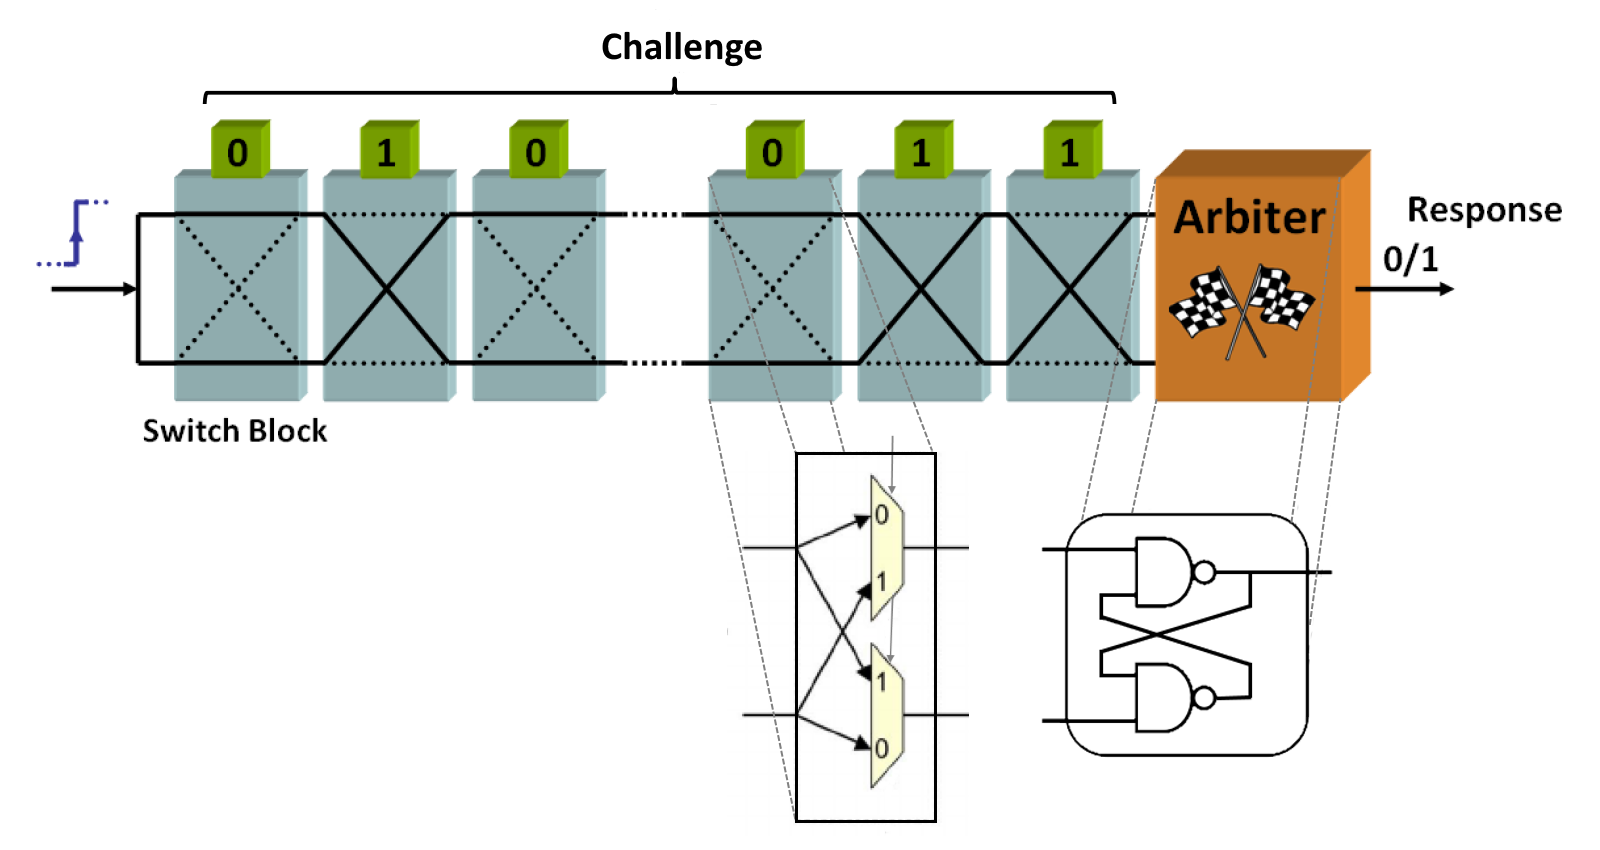
\includegraphics[width=0.9\textwidth]{images/arbiter_4.png}}
	\caption{Construction of a basic arbiter PUF, \emph{switching blocks} realized with muxes and a \emph{SR latch} realized with NAND gates, modified graphic based on [seb 34]}
	\label{img:1}
\end{figure}

\textbf{\emph{Security Issues:}}
Though the challenge set is large still the number of delay paramerters which effect the PUF response are linear in n, hence the 2$^n$ challenges cannot generate independant reponses. A certain model or mathematical clone can be build for a given arbiter PUF if adversary learns the underlying delay parameters. This clone can accurately forecast the PUF reponse rendering the arbiter PUF hackable in security applications scenarios. Machine learning techniques like artificial neural
networks (ANNs) and support-vector machines (SVMs) can be employed to implicitly learn the underlying delay parameters by observing the challenge response pairs.

\subsubsection{SRAM PUFs}
\label{srampufs}

Static Random-Access Memory (SRAM) is a digital memory technology based on bistable circuits. [seb 34 section 2.4.4.]. Refer to fig [ ] for details of an SRAM cell. It consists of six MOSFETs transistors, out of which four are contained in two invertors. Each invertor comprises of one p-MOS and one n-MOS MOSFET. As you can see from fig [ ] the invertors are cross-coupled at SRAMs cell core. In logic sense, the circuit has two stable states (bistable), each state represented by a binary
digit (0 or 1) that is stored in the cell. Two MOSFETs are used to read and write the cell contents. An SRAM cell is volatile and does not store its state on power-off.\\

There are three possible operating points, two are stable and one is metastable fig [ ]. The deviation from stable points is automatically restored to its original point due to the feedback from the circuit. Adversely any deviation from metastable point is amplified by the positive feedback from the circuit and cell moves to either of the stable points. After the supply voltage $V_{DD}$ comes up the cell shifts to one of the preferred stable points, which is determined by the difference in
strength (device mismatch) of the MOSFETs in the cross-coupled invertor circuit. Due to performance and efficiency reasons the invertors are designed to be perfectly in sync, the device mismatch is a result of the random process variations in the silicon production process. This random preferred intial operating point is unique a specfic cell. For small mismatch the preferred initial stable point is determined by sign of the mismatch, though voltage noise can render the cell to
power-up in a non-preferred state. Finally the cells with almost zero mismatch power-up in metastable state and shift to one of the stable points randomly.\\

Most SRAM cells have strongly preferred cell-specific initial state due to the magnitude of the process variations on the device mismatch, only a small number of the cells have weak preferred or no preferred state, hence a typical SRAM cell exhibits strong PUF behavior. These cells are arranged in a large array giving millions of reponse bits, challenge for this cell assembly is the address of the cell.\\

\subsubsection{Ring Oscillator PUF}

Proposed by Gassend et al. [ ] it is another type of delay-based intrinsic PUF. There are two parts to ring oscillator PUF, first is the ring oscillator and other is the frequency counter which are arranged is a configuration as shown in the fig. [ ] and connected to a response generating algorithm. Gassend et al. uses a variant of the switch block base delay line similar to arbiter PUF \ref{arbiterpuf} which is transformed in a oscillator with the help of a negative feedback.
An AND gate is added to turn off/on the oscillation, which is fed to a frequency counter that counts the number of oscillating cycles in a fixed time interval. A same setup for ring oscillator on another device with same implementation has different counter value because of the silicon process variations which forms the basis of the PUF reponse.\\

\begin{figure}
\centering
\fbox{ 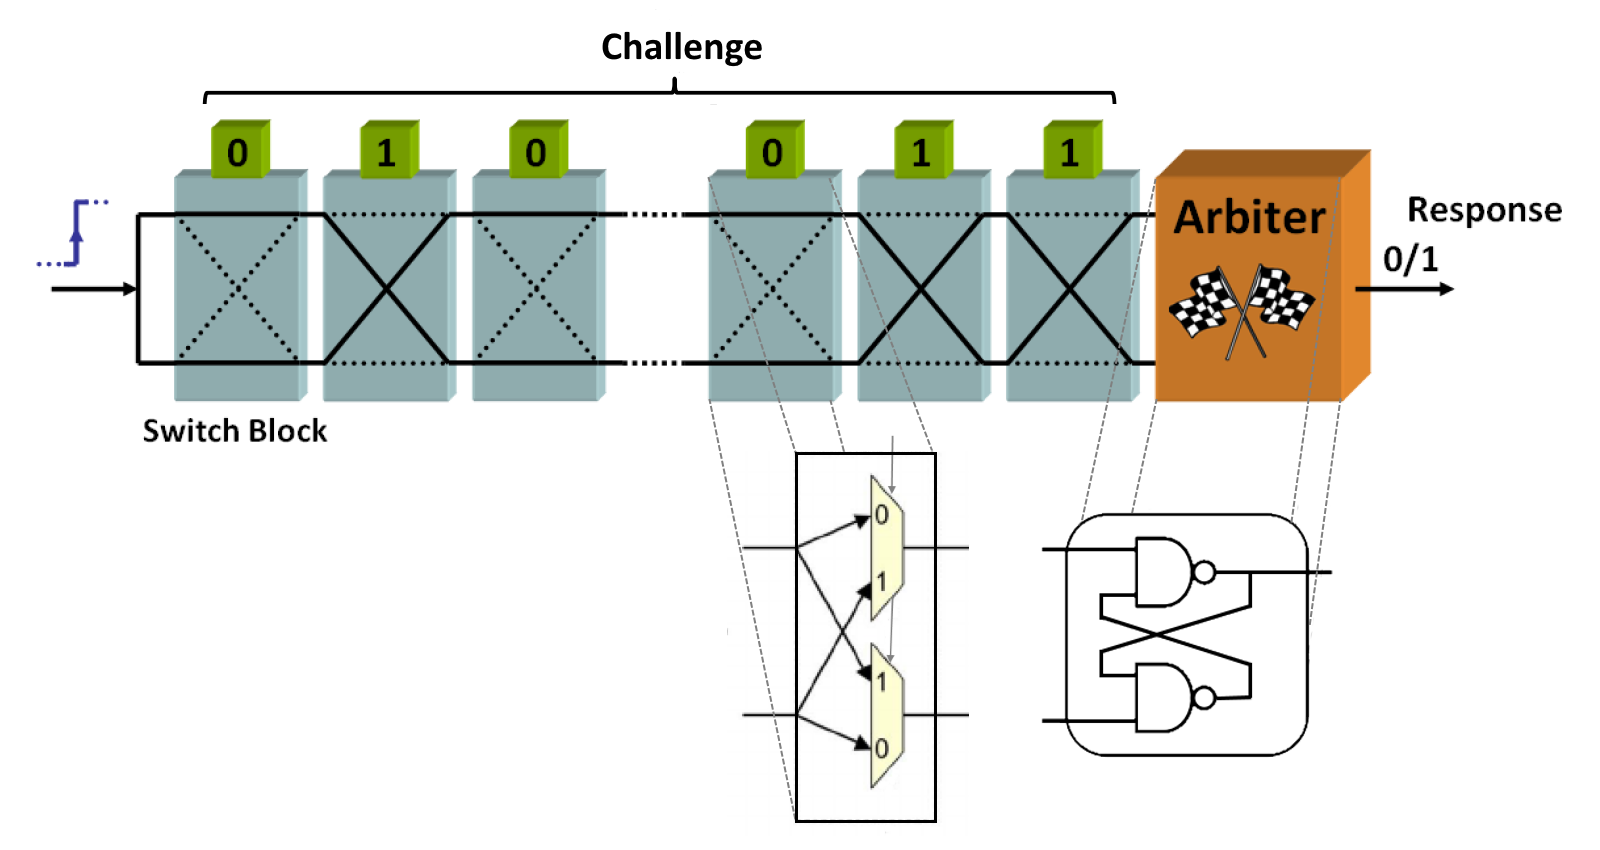
\includegraphics[width=0.9\textwidth]{images/arbiter_4.png}}
\caption{Construction of a basic ring oscillator PUF, modified graphic based on [seb 34]} 
\label{img:2}
\end{figure}

There are some other side effects associated with ring oscillator PUFs, one of them is significant influence from the environmental conditions like temperature changes and voltage fluctuations. The frequency changes introduced by these factors outweigh the deviations caused by the process variations, so to counteract these changes we need a post processing technique known as \emph{compensated measuring}. The main idea is to calculate the ratio of the frequency of two ring oscillators
on the same device since they both are affected with identical environmental factors, hence the ratio would be more uniform. According to observations average intra-distance distance between evaluations is approximately less than the average inter-distance by 50\% [seb 34 section 2.4.2] 

\subsubsection{Optical PUFs}

Even before the introduction of PUFs an unclonable identification system based on random optical reflection patterns was proposed in [th 53 section 3.1.1]. Proposed by Pappu et al. as Physical one-way functions (POWF) optical PUF contains a microstructure constructed by blending microscopic (500 $\mu$m) refractive glass spheres in a miniature (10 x 10 x 2.54 $mm$) transparent epoxy plate. This token is illuminated with a helium neon laser which produces a irregular wavefront,
the cause for this irregularity is the multiple scattering of the laser by the refractive particles. Finally a CCD camera captures the speckle pattern and digitally processed by applying Gabor Hash to it as a feature extraction procedure. [th section 3.1.1] The final output is a string of bits that deviates significantly if the orientation of the laser beam is even minutely changed.\\

Challenge is made up from the exact positioning of the laser and the resulting Gabor hash of the emerged speckle pattern is considered as response. The operation and implemetation for optical PUF is shown in fig [ ]. Number of experiments were performed by [th 41 42] for testing the characterstics of the optical PUF and following summarizes their results. These values are taken from the [pappu et al. and th 42]. Total four optical tokens used with 576 individual challenges, for the
responses intra and inter distance measures were evaluated with average inter-distance of $\mu_{inter}$ = 49.79\% and average intra-distance of 
$\mu_{intra}$ = 25.25\%. One of the main limitation of such an optical PUF is the burdensome large setup consisting of a laser and mechanical positioning system. They are classified as Non-electronic, non-intrinisic and strong PUFs.\\

\begin{figure}
\centering
\fbox{ 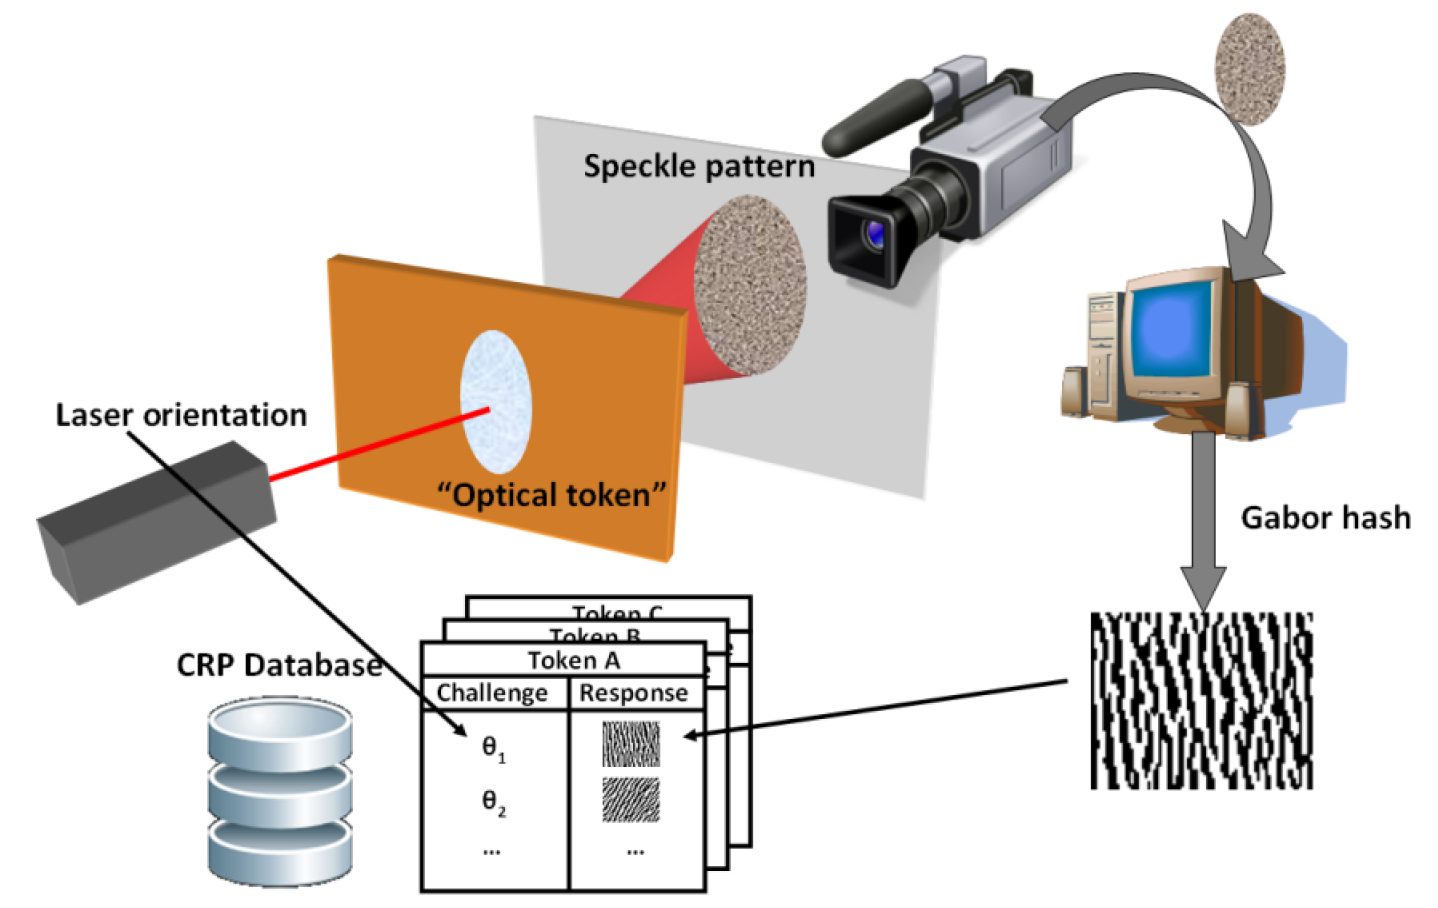
\includegraphics[width=0.9\textwidth]{images/opticalPUF.png}}
\caption{Construction of a basic optical PUF as proposed by Pappu et al. \cite{18,19}.}
\label{img:3}
\end{figure}

\section{Fuzzy extractors}

\section{linear codes, bch , golay}

\section{Jaccard index}

\section{Congnicrypt Syonpsis}

